% file: HT-pattern.tex

\documentclass[tikz]{standalone}
\usetikzlibrary{decorations.pathreplacing, positioning, arrows.meta, shapes.multipart}

\begin{document}
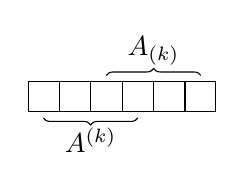
\begin{tikzpicture}[P/.style = {rectangle split, rectangle split parts = 6, rectangle split horizontal, 
  	draw, anchor = center}]
  \node[P] (pattern) {};

  \draw[decoration = {brace, mirror, raise = 2pt}, decorate] (pattern.one south) -- node[below = 2pt] {$A^{(k)}$} (pattern.four south);
  \draw[decoration = {brace, raise = 2pt}, decorate] (pattern.three north) -- node[above = 2pt] {$A_{(k)}$} (pattern.six north);
\end{tikzpicture}
\end{document}

